\chapter{Spektrales Lernen auf Graphen}
\label{spektrales_lernen}

Das spektrale Lernen auf Graphen \bzw{} die Formulierung eines spektralen Faltungsoperator auf Graphen basiert auf der spektralen Graphentheorie, \dhe{} der Betrachtung des Spektrums eines Graphen definiert über dessen Eigenwerte.
Merkmale auf den Knoten eines Graphen können über das Spektrum analog zur Fourier-Transformation in dessen Frequenzraum zerlegt und wieder retransformiert werden.
Diese Transformation erlaubt damit die fundamentale Formulierung eines Faltungsoperators in der spektralen Domäne des Graphen.
Da der so definierte spektrale Faltungsoperator insbesondere rotationsinvariant ist, wird dieser im Verlauf des Kapitels für den Kontext von Graphen im euklidschen Raum modifiziert.

Durch die spektrale Formulierung kann weiterhin ein effizientes Pooling auf Graphen formuliert werden, welches uns erlaubt, Netzarchitekturen auf Graphen völlig analog zu klassischen \glspl{CNN} auf zweidimensionalen Bildern zu generieren.

\section{Spektrale Graphentheorie}
\label{spektrale_graphentheorie}

Es gibt 2 große Quellen hier:
\begin{itemize}
  \item Spectral Graph Theory by Chung
  \item Discrete Laplace-Beltrami Operator
\end{itemize}
+ 5 zum Lernen:
\begin{itemize}
  \item Semi Supervised Classification
  \item Fast Localized Spectral Filterung
  \item Wavelets on Graphs via Spectral Graph Theory
  \item The Emerging Field of Signal Processing on Graphs
  \item How powerful are Graph Convolutions? (Review)
\end{itemize}

\subsection{Eigenwerte und Eigenvektoren reell symmetrischer Matrizen}
\label{eigenwerte_symmetrischer_matrizen}

\todo{intro}

$\ma{M} \in \gls{R}^{N \times N}$.
$\gls{eiv} \in \gls{R}^{N}$, $\gls{eiv} \neq \mathbf{0}$.
$\gls{lambda} \in \gls{R}$.
\emph{Eigenwertproblem} $\ma{M}\gls{eiv} = \gls{lambda}\gls{eiv}$.
Zu einem \emph{Eigenwert} $\gls{lambda}$ gibt es unendlich viele (skalierte) \emph{Eigenvektoren} \gls{eiv}.
Wir definieren den Eigenvektor \gls{eiv} eines Eigenwertes \gls{lambda} daher eindeutig über die Bedingung $\left\|\gls{eiv}\right\|_2 = 1$.
Sei \ma{M} weiterhin symmetrisch, \dhe{} $\ma{M} = \ma{M}^{\top}$.
Dann gilt für zwei unterschiedliche Eigenvektoren $\gls{eiv}_1$ und $\gls{eiv}_2$, dass $\gls{eiv}_1 \gls{ortho} \gls{eiv}_2$.
Weiterhin hat \ma{M} genau $N$ reelle Eigenwerte mit ${\left\{\gls{lambda}_i\right\}}_{i=1}^N$.

Wir definieren zu \ma{M} die orthogonale \emph{Eigenvektormatrix} $\gls{Eiv} \coloneqq \left[\gls{eiv}_1, \ldots, \gls{eiv}_n\right] \in \gls{R}^{N \times N}$, wobei $\gls{Eiv}\gls{Eiv}^{\top}=\gls{I}$, und dessen korrespondierende Eigenwertdiagonalmatrix $\gls{Lambda} \coloneqq \gls{diag}\left({\left[\gls{lambda}_1, \ldots, \gls{lambda}_N\right]}^{\top}\right)$, \dhe{} $\gls{Lambda}_{ii} = \gls{lambda}_i$.
Dann gilt $\ma{M}\gls{Eiv} = \gls{Eiv}\gls{Lambda}$ und insbesondere ist \ma{M} diagonalisierbar über
\begin{equation*}
  \ma{M} = \ma{M}\gls{Eiv}\gls{Eiv}^{\top} = \gls{Eiv}\gls{Lambda}\gls{Eiv}^{\top}.
\end{equation*}

Weiterhin gilt für die $k$te Potenz von $\ma{M}$, $k \in \gls{N}$,
\begin{equation}
  \ma{M}^k = {\left(\gls{Eiv}\gls{Lambda}\gls{Eiv}^{\top}\right)}^k = \gls{Eiv}\gls{Lambda}^k\gls{Eiv}^{\top}.
  \label{eq:matrix_potenz}
\end{equation}

Dieser Zusammenhang lässt sich verdeutlichen, wenn man die Potenz ausschreibt:
\begin{equation*}
  {\left(\gls{Eiv}\gls{Lambda}\gls{Eiv}^{\top}\right)}^k = \gls{Eiv}\gls{Lambda}\gls{Eiv}^{\top}\gls{Eiv}\gls{Lambda}\gls{Eiv}^{\top}\prod^{k-2}_{i=1} \gls{Eiv}\gls{Lambda}\gls{Eiv}^{\top} = \gls{Eiv}\gls{Lambda}^2\gls{Eiv}^{\top} \prod^{k-2}_{i=1} \gls{Eiv}\gls{Lambda}\gls{Eiv}^{\top} = \gls{Eiv}\gls{Lambda}^k \gls{Eiv}^{\top}.
\end{equation*}

Falls \ma{M} weiterhin \emph{schwach diagonaldominant} ist, \dhe{}
\begin{equation}
  \sum_{\substack{j=1\\j \neq i}}^N \left|\ma{M}_{ij}\right| \leq \left|\ma{M}\right|_{ii},
  \label{eq:schwach_diagonaldominant}
\end{equation}
und weiterhin $\ma{M}_{ii} \geq 0$ für alle $i \in \left\{1, \ldots, N\right\}$, dann ist \ma{M} \emph{positiv semidefinit}, \dhe{} $\ve{x}^{\top}\ma{M}\ve{x} \geq 0$ für alle $\ve{x} \in \gls{R}^{N}$.
Eigenwerte symmetrischer positiv semidefiniter Matrizen $\lambda_i \in \gls{R+}$ sind positiv reell und es lässt sich folglich auf diesen eine Ordnung definieren mit $0 \leq \gls{lambda}_1 \leq \cdots \leq \gls{lambda}_N \coloneqq \gls{lambdamax}$.

\todo{quelle}

\subsection{Laplace-Matrix}
\label{laplace_matrix}

Our eigenvalues relate well to other graph invariants for general graphs in a way that other definitions (such as the eigenvalues of adjacency matrices) often fail to do.
The advantages of this definition are perhaps due to the fact that it is consistent with the eigenvalues in spectral geometry and in stochastic processes.
Many results which were only known for regular graphs can be generalized to all graphs~\cite{Chung}.

\todo{intro}

Für einen schleifenlosen, ungerichteteten, gewichtet oder ungewichteten Graphen \gls{G} und dessen Adjazenzmatrix \gls{A} mit Gradmatrix \gls{D} ist die \emph{kombinatorische Laplace-Matrix} \gls{L} definiert als $\gls{L} \coloneqq \gls{D} - \gls{A}$~\cite{Chung}.
Die \emph{normalisierte Laplace-Matrix} \gls{Lnorm} ist definiert als $\gls{Lnorm} \coloneqq \gls{D}^{-\frac{1}{2}} \gls{L} \gls{D}^{-\frac{1}{2}}$ mit der Konvention, dass $\gls{D}^{-\frac{1}{2}}_{ii} = 0$ für isolierte Knoten $\gls{v}_i \in \gls{V}$ in \gls{G}, \dhe{} $\gls{D}_{ii} = 0$~\cite{Chung}.
Daraus ergibt sich die elementweise Definition
\begin{equation*}
  \gls{Lnorm}_{ij} \coloneqq \begin{cases}
  1, & \text{wenn }i = j,\\
    -\frac{\gls{w}\left(\gls{v}_i, \gls{v}_j\right)}{\sqrt{\gls{d}\left(\gls{v}_i\right)\gls{d}\left(\gls{v}_j\right)}}, & \text{wenn }\gls{v}_i \gls{adj} \gls{v}_j,\\
  0, & \text{sonst.}
\end{cases}
\end{equation*}
Für verbundene Graphen kann \gls{Lnorm} vereinfacht werden zu $\gls{Lnorm} \coloneqq \gls{I} - \gls{D}^{-\frac{1}{2}} \gls{A} \gls{D}^{-\frac{1}{2}}$~\cite{Chung}.
Jeder Eintrag auf der Diagonalen der normalisierten Laplace-Matrix ist folglich Eins.
\gls{Lnorm} ist damit normalisiert auf den (gewichteten) Grad zweier adjazenter Knoten $\gls{v}_i$ und $\gls{v}_j$.
Es ist anzumerken, dass \gls{L} und insbesondere \gls{Lnorm} symmetrisch sind, wohingegen eine Normalisierung der Form $\gls{D}^{-1}\gls{L}$ dies in der Regel nicht wäre~\cite{Reuter}.

\gls{L} und \gls{Lnorm} sind keine ähnlichen Matrizen.
Insbesondere sind ihre Eigenvektoren unterschiedlich.
Die Nutzung von \gls{L} oder \gls{Lnorm} ist damit abhängig von dem Problem, welches man betrachtet~\cite{Hammond}.
Wir schreiben \gls{Lboth} wenn die Wahl der Laplace-Matrix, ob \gls{L} oder \gls{Lnorm}, für die weitere Berechnung zwar fest, aber irrelevant ist.

\paragraph{Interpretation}
\label{laplace_interpretation}

\todo{kurz laplace beltrami}

Sei $\ve{f} \in \gls{R}^N$ eine Funktion \bzw{} ein Signal auf den Knoten eines Graphen \gls{G}.
Dann kann für die kombinatorische Laplace-Matrix \gls{L} verifiziert werden, dass \gls{L} die Gleichung
\begin{equation*}
  {\left(\gls{L}\ve{f}\right)}_i = \sum_{i \gls{adj} j} \gls{w}\left(\gls{v}_i, \gls{v}_j\right) \left(\ve{f}_i - \ve{f}_j\right)
\end{equation*}
erfüllt~\cite{Hammond}.
Sei $\gls{G}$ nun ein Graph, der aus einem (unendlichen) zweidimensionalen regulärem Gitter entstanden ist, \dhe{} jeder Knoten $\gls{v}_i$ besitzt genau $4$ Nachbarn mit gleichen Kantengewichten $\frac{1}{\delta^2}$, wobei $\delta \in \gls{R}$ beliebige Konstante.
Zur einfacheren Veranschaulichung benutzen wir dabei für die Signalstärke $\ve{f}_i$ eines Knoten $v_i$ an Position $\left(x, y\right)$ die Indexnotation $\ve{f}_{x,y}$.
Dann beschreibt
\begin{equation*}
  {\left(\gls{L}\ve{f}\right)}_{x,y} = \frac{4\ve{f}_{x,y} - \ve{f}_{x+1,y} - \ve{f}_{x-1,y} - \ve{f}_{x,y+1} - \ve{f}_{x,y-1}}{h^2}
\end{equation*}
die \emph{5-Punkte-Stern} Approximation $-\nabla^2 f$ (bei umgekehrtem Vorzeichen) definiert auf den Punkten $\left\{\left(x,y\right), \left(x+\delta,y\right), \left(x-\delta,y\right), \left(x,\delta+h\right),\left(x,y-\delta\right)\right\}$~\cite{Hammond}.\todo{grafik}
Ähnlich zu einem regulären Gitter lässt sich ein Graph \gls{G} auch über beliebig viele Abtastpunkte einer differenzierbaren Mannigfaltigkeit konstruieren.
Es zeigt sich, dass mit steigender Abtastdichte und geeigneter Wahl der Kantengewichte die normalisierte Laplace-Matrix \gls{Lnorm} zu dem kontinuierlichem Laplace-Beltrami Operator konvergiert~\cite{Hammond}.
Damit kann $\gls{Lnorm}$ als die diskrete Analogie des $\nabla^2$ Operators auf Graphen verstanden werden.
Der Laplace-Beltrami Operator misst dabei, in wie weit sich eine Funktion $f$ an einem Punkt $x$ von dem Durchschnitt aller Funktionspunkte um einen kleinen Bereich um $x$ unterscheidet.
Die Laplace-Matrix operiert dabei völlig analog, in dem sie misst, wie sehr sich eine (diskrete) Funktion um einen Knoten im Vergleich zu seinen Nachbarknoten unterscheidet.

Eigenwerte und Eigenvektoren von \gls{Lboth} helfen uns dabei, die lineare Transformation einer Funktion \ve{f} (mehrfach) angewendet auf \gls{Lboth} besser zu verstehen.
Wir können dafür \ve{f} als Linearkombination der Eigenbasis $\sum_i c_i \gls{eiv}_i$ schreiben und erhalten
\begin{equation*}
  \gls{Lboth}^k \ve{f} = \sum_i c_i \gls{Lboth}^k \gls{eiv}_i = \sum_i c_i \gls{lambda}_i^k \gls{eiv}_i.
\end{equation*}
Somit können Eigenschaften von \gls{Lboth} und damit des Graphen selber durch dessen Eigenwerte und Eigenvektoren beschrieben werden.

\paragraph{Eigenschaften}
\label{laplace_eigenschaften}

$\gls{Lboth} \in \gls{R}^{N \times N}$ ist eine reell symmetrisch, positiv semidefinite Matrix~\cite{Chung}.
Folglich besitzt \gls{Lboth} nach Kapitel~\ref{eigenwerte_symmetrischer_matrizen} genau $N$ positiv reelle Eigenwerte ${\left\{\gls{lambda}_i\right\}}_{i=1}^N$ mit Ordnung $0 \leq \gls{lambda}_1 \leq \cdots \leq \gls{lambda}_N$ und $N$ korrespondierende orthogonale Eigenvektoren ${\left\{\gls{eiv}_i\right\}}_{i=1}^N$.

Die kombinatorische Laplace-Matrix $\gls{L}$ ist nach~\eqref{eq:schwach_diagonaldominant} weiterhin schwach diagonaldominant.
Insbesondere summiert sich jede Reihen- und Spaltensumme von \gls{L} zu Null auf, \dhe{} $\sum_{j=1}^N \gls{L}_{ij} = \sum_{j=1}^N \gls{L}_{ji} = 0$.
Daraus folgt unmittelbar, dass $\gls{lambda}_1 = 0$, da $\gls{eiv}_1 = \frac{1}{\sqrt{N}}{\left[1, \ldots, 1\right]}^{\top} \in \gls{R}^N$ Eigenvektor von \gls{L} mit $\gls{L}\gls{eiv}_1 = \ve{0}$.
\gls{Lnorm} hingegen ist nicht zwingend schwach diagonaldominant.
Es lässt sich jedoch zeigen, dass auch für \gls{Lnorm} gilt, dass $\gls{lambda}_1 = 0$~\cite{Chung}.

Eine der interessantesten Eigenschaften eines Graphs ist dessen Konnektivität.
Die Laplace-Matrix \gls{Lboth} \bzw{} dessen Eigenwerte stellen ein geeignetes Mittel zur Untersuchung dieser Eigenschaft dar.
So gilt \zB{} für einen verbundenen Graphen \gls{G}, dass $\gls{lambda}_2 > 0$.
Falls $\gls{lambda}_i = 0$ und $\gls{lambda}_{i+1} \neq 0$, dann besitzt $\gls{G}$ genau $i$ verbundene Komponenten~\cite{Chung}.
Damit ist die Anzahl der Null-Eigenwerte äquivalent zu der Anzahl an Komponenten, die ein Graph besitzt.
Für \gls{Lnorm} lässt sich weiterhin zeigen, dass $\gls{lambdamax} \leq 2$ eine obere Schranke ihrer Eigenwerte ist~\cite{Chung}.

Aus der Laplace-Matrix können ebenso Rückschlüsse über die kürzeste Pfaddistanz zweier Knoten gewonnen werden.
So gilt für $\gls{Lboth}^{k}$ mit $k \in \gls{N}$, dass $\gls{Lboth}^k_{ij} = 0$ genau dann, wenn $\gls{s}\left(v_i, v_j\right) > k$~\cite{Hammond}.
Damit beschreibt $\gls{Lboth}^k_i$ bildlich gesprochen die Menge an Knoten, die maximal $k$ Kanten von $i$ entfernt liegen.

\section{Spektraler Faltungsoperator}
\label{spektraler_faltungsoperator}

\subsection{Graph-Fourier-Transformation}
\label{graph_fourier_transformation}

\subsection{Polynomielle Approximation}
\label{polynomielle_approximation}

\paragraph{Tschebyschow-Polynome}
\label{tschebyschow_polynome}

\section{Graph Convolutional Networks}
\label{graph_convolutional_networks}

\citeauthor{gcn} motivieren einen weiteren Ansatz zur Faltung auf Graphen, genannt \emph{\gls{GCN}}, der auf der Methodik des spekralen Faltungsoperators aus Kapitel~\ref{spektraler_faltungsoperator} aufbaut und dabei wie eine \enquote{differenzierbare und parametrisierte Generalisierung des eindimensionalen Weisfeiler-Lehman Algorithmus auf Graphen} fungiert~\cite{gcn}.

\paragraph{Faltungsoperator}
\label{gcn_faltungsoperator}

Sei $\ve{f}_{\mathrm{in}} \star \ve{\hat g} \approx \sum_{k=0}^K c_k \gls{T}_k\left(\gls{Lbothtilde}\right) \ve{f}_{\mathrm{in}}$ der in~\eqref{eq:tschebyschow_faltung_L} definierte spektrale Faltungsoperator mit $K=1$.
Dann ist $\ve{f}_{\mathrm{in}} \star \ve{\hat g}$ eine lineare Funktion \bzgl{} \gls{Lboth} und damit eine lineare Funktion auf dem Spektrum des Graphen~\cite{gcn}.
Mit $K=1$ betrachtet der spektrale Faltungsoperator nur noch die lokale Nachbarschaft eines jeden Knotens (\vgl{}~\ref{polynomielle_approximation}).
Es ist anzumerken, dass dies in der Regel keinen Nachteil darstellt.
So hat es sich bei gegenwärtigen \enquote{State-of-the-Art}-\glspl{CNN} auf Bildern ebenfalls eingebürgert, nur noch über minimale $3\times3$ Filtergrößen zu falten und stattdessen Merkmale weit entfernterer Knoten über die mehrfache Aneinanderreihung der Faltungsschichten mittels tieferer Netze zu gewinnen~(\vgl{}~\cite{gcn, vgg, He}).
Unter dieser Restriktion vereinfacht sich $\ve{f}_{\mathrm{in}} \star \ve{\hat g}$ zu
\begin{equation}
  \ve{f}_{\mathrm{in}} \star \ve{\hat g} \approx c_0\, \ve{f}_{\mathrm{in}} + c_1 \left(\frac{2}{\gls{lambdamax}}\gls{Lboth} - \gls{I}\right)\ve{f}_{\mathrm{in}}
  \label{eq:gcn_faltung_both}
\end{equation}
mit zwei freien Parametern $c_0$ und $c_1$~\cite{gcn}.
Für $\gls{Lnorm}$ auf einem zusammenhängenden Graphen \gls{G} gilt dann nach~\eqref{eq:gcn_faltung_both} weiter
\begin{equation}
  \ve{f}_{\mathrm{in}} \star \ve{\hat g} \approx c_0 \, \ve{f}_{\mathrm{in}} + c_1 \left(\gls{Lnorm} - \gls{I}\right)\ve{f}_{\mathrm{in}} = c_0 \, \ve{f}_{\mathrm{in}} - c_1 \gls{D}^{-\frac{1}{2}} \gls{A} \gls{D}^{-\frac{1}{2}} \ve{f}_{\mathrm{in}},
  \label{eq:gcn_faltung_norm}
\end{equation}
wobei $\gls{lambdamax} \coloneqq 2$ auf dessen obere Schranke gesetzt wird~\cite{gcn}.
Um die Gefahr des Overfittings und die Anzahl an Berechnungen pro Schicht weiter zu beschränken, reduziert sich~\eqref{eq:gcn_faltung_norm} mit einem einzigen Parameter $c \coloneqq c_0$ mit $c = -c_1$ zu~\cite{gcn}
\begin{equation*}
  \ve{f}_{\mathrm{in}} \star \ve{\hat g} \approx c \left(\gls{I} + \gls{D}^{-\frac{1}{2}} \gls{A} \gls{D}^{-\frac{1}{2}} \right) \ve{f}_{\mathrm{in}}.
\end{equation*}
Die skalierten Eigenwerte von \gls{Lambdatilde} liegen auf Grund der Addition mit \gls{I} nun im Intervall $\left[0, 2\right]$ (\vgl{}~\cite{gcn}).
Demnach können wiederholte Anwendungen des Faltungsoperators zu \enquote{numerischen Instabilitäten und folglich zu explodierenden oder verschwindenen Gradienten} führen~\cite{gcn}.
\citeauthor{gcn} führen zur Behebung dieses Problems die folgende Renormalisierung durch: $\gls{I} + \gls{D}^{-1/2} \gls{A} \gls{D}^{-1/2} \rightarrow \gls{Dtilde}^{-1/2} \gls{Atilde} \gls{Dtilde}^{-1/2}$ mit $\gls{Atilde} \coloneqq \gls{A} + \gls{I}$ und $\gls{Dtilde}_{ii} \coloneqq \sum_{j=1}^N \gls{Atilde}_{ij}$.
Der entgültige Faltungsoperator des \glspl{GCN} ergibt sich dann als
\begin{equation}
  \ve{f}_{\mathrm{in}} \star \ve{\hat g} \approx c\, \gls{Dtilde}^{-\frac{1}{2}} \gls{Atilde} \gls{Dtilde}^{-\frac{1}{2}} \ve{f}_{\mathrm{in}}
  \label{eq:gcn_renorm}
\end{equation}
auf einem einzigen freien Parameter $c \in \gls{R}$.

\paragraph{Implementierung}
\label{gcn_tensor}

Die Faltung des \glspl{GCN} auf Merkmalsmatrizen lässt sich analog zur Tensorimplementierung des spektralen Faltungsoperators in Kapitel~\ref{polynomielle_approximation} beschreiben, mit dem Unterschied, dass wir aufgrund der Festlegung von $K=1$ keinen Filtertensor, sondern lediglich eine Filtermatrix $\gls{W} \in \gls{R}^{M_{\mathrm{in}} \times M_{\mathrm{out}}}$ nutzen.
Die Faltung einer Eingabemerkmalsmatrix $\gls{F}_{\mathrm{in}} \in \gls{R}^{N \times M_{\mathrm{in}}}$ auf eine Ausgabemerkmalsmatrix $\gls{F}_{\mathrm{out}} \in \gls{R}^{N \times M_{\mathrm{out}}}$ ergibt sich dann als
\begin{equation}
  \ma{F}_{\mathrm{out}} \coloneqq \gls{Dtilde}^{-\frac{1}{2}} \gls{Atilde} \gls{Dtilde}^{-\frac{1}{2}}\, \ma{F}_{\mathrm{in}} \gls{W}
  \label{eq:gcn_tensor}
\end{equation}
mit Faltungsaufwand $\gls{O}\left(M_{\mathrm{in}}M_{\mathrm{out}}\left|\gls{E}\right|\right)$, weil $\gls{Atilde}\ma{F}_{\mathrm{in}}$ effizient mit der Multiplikation einer dünnbesetzten mit einer dichtbesetzten Matrix implementiert werden kann~\cite{gcn}.

\paragraph{Beziehung zum Weisfeiler-Lehman Algorithmus}
\label{weisfeiler_lehman_beziehung}

\begin{algorithm}[t]
\centering
\begin{algorithmic}
  \REQUIRE{} Initiale Knotenfärbung $\ve{h}^{\left(0\right)} \in \gls{R}^N$
  \ENSURE{} Finale Knotenfärbung $\ve{h}^{\left(T\right)} \in \gls{R}^N$ nach $T$ Durchläufen
  \STATE{} $t \leftarrow 0$
  \REPEAT{}
    \FOR{$\gls{v}_i \in \gls{V}$}
      \STATE{} $\ve{h}^{\left(t+1\right)}_i \leftarrow \mathrm{hash}\left(\sum_{\gls{v}_j \in \gls{Neighbor}\left(\gls{v}_i\right)} \ve{h}^{\left(t\right)}_j\right)$
    \ENDFOR{}
    \STATE{} $t \leftarrow t + 1$
  \UNTIL{Konvergenz}
\end{algorithmic}
  \caption[Weisfeiler-Lehman Algorithmus]{Eindimensionaler Weisfeiler-Lehman Algorithmus auf einer initialen Knotenfärbung $\ve{h}^{\left(0\right)} \in \gls{R}^N$ eines Graphen \gls{G} mit $\gls{v}_i \in \gls{Neighbor}\left(\gls{v}_i\right)$~\cite{wl}.}
\label{alg:wl}
\end{algorithm}

Der \emph{eindimensionale Weis\-fei\-ler-Lehman Algorithmus} beschreibt eine weit-untersuchte Methode zur Knotenklassifizierung eines Graphen basierend auf einer intialen Färbung \bzw{} Merkmalsverteilung auf den Knoten eines Graphen \gls{G}, die unteranderem zur Bestimmung von Graphisomorphismen genutzt wird~\cite{douglas}.
Basierend auf einer intialen Knotenfärbung $\ve{h}^{\left(0\right)} \in \gls{R}^N$ wird die Farbe eines jeden Knotens $\gls{v}_i \in \gls{V}$ sukzessive mit Hilfe einer Hashfunktion $\mathrm{hash}\left(\cdot\right)$ so angepasst, dass sie die vorangegangene Farbe des Knotens zusammen mit den Farben seiner lokalen Nachbarschaft repräsentiert.
Dieser Prozess wiederholt sich solange, bis eine stabile Knotenfärbung gefunden wurde, \dhe{} die gefundene Färbung des Graphen konvergiert (\vgl{} Algorithmus~\ref{alg:wl}).

Sei die Hashfunktion gegeben als eine differenzierbare, nicht-lineare Aktivierungsfunktion $\gls{act}\left(\cdot\right)$ eines neuronalen Netzes.
Dann ergibt sich die Faltung des \glspl{GCN} als
\begin{equation*}
  \ve{h}^{\left(t+1\right)}_i = \gls{act}\left(\sum_{\gls{v}_j \in \gls{Neighbor}\left(\gls{v}_i\right)} \frac{1}{\sqrt{d_i d_j}} \ve{h}^{\left(l\right)}_j \gls{W} \right),
\end{equation*}
wobei $1/\sqrt{d_i d_j} \in \gls{R}$ eine Normalisierungskonstante für die Kante $\left(\gls{v}_i, \gls{v}_j\right) \in \gls{E}$ ist~\cite{gcn}.
Damit kann die Faltung des \glspl{GCN} als \enquote{differenzierbare und parametrisierte Generalisierung des eindimensionalen Weisfeiler-Lehman Algorithmus auf Graphen} verstanden werden~\cite{gcn}.

\begin{figure}[t]
\centering
  \subfigure[$\gls{G}_0$]{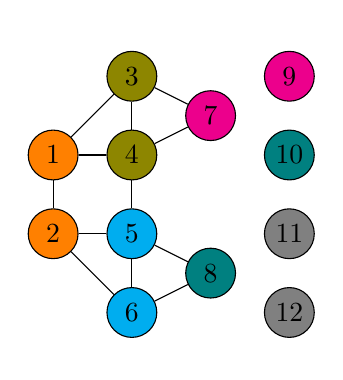
\begin{tikzpicture}
  \fill [white] (-1, -2) rectangle (1, 2) node {};  % Zentriere Graph.
  \tikzstyle{node}=[circle,draw, minimum width=18pt, inner sep=0pt, fill=white]
  \tikzstyle{color1}=[fill=orange]
  \tikzstyle{color2}=[fill=olive]
  \tikzstyle{color3}=[fill=cyan]
  \tikzstyle{color4}=[fill=magenta]
  \tikzstyle{color5}=[fill=teal]
  \tikzstyle{color6}=[fill=gray]

  \node[node, color1] (1)  at (-2, 0.5)  {$1$};
  \node[node, color1] (2)  at (-2, -0.5) {$2$};
  \node[node, color2] (3)  at (-1, 1.5)  {$3$};
  \node[node, color2] (4)  at (-1, 0.5)  {$4$};
  \node[node, color3] (5)  at (-1, -0.5) {$5$};
  \node[node, color3] (6)  at (-1, -1.5) {$6$};
  \node[node, color4] (7)  at (0,  1)    {$7$};
  \node[node, color5] (8)  at (0,  -1)   {$8$};

  \node[node, color4] (9)  at (1, 1.5)   {$9$};
  \node[node, color5] (10) at (1, 0.5)   {$10$};
  \node[node, color6] (11) at (1, -0.5)  {$11$};
  \node[node, color6] (12) at (1, -1.5)  {$12$};

  \path (1) edge (2);
  \path (1) edge (3);
  \path (1) edge (4);
  \path (2) edge (5);
  \path (2) edge (6);
  \path (3) edge (4);
  \path (3) edge (7);
  \path (4) edge (5);
  \path (4) edge (7);
  \path (5) edge (6);
  \path (5) edge (8);
  \path (6) edge (8);
\end{tikzpicture}
}
\hspace{1cm}
  \subfigure[$\gls{G}_1$]{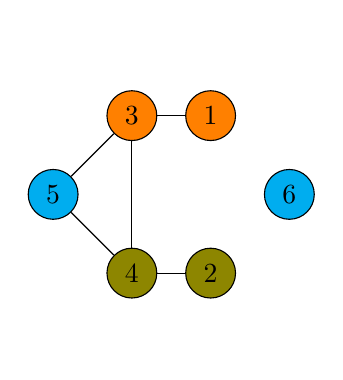
\begin{tikzpicture}
  \fill [white] (-1, -2) rectangle (1, 2) node {};  % Zentriere Graph.
  \tikzstyle{node}=[circle,draw, minimum width=18pt, inner sep=0pt, fill=white]
  \tikzstyle{color1}=[fill=orange]
  \tikzstyle{color2}=[fill=olive]
  \tikzstyle{color3}=[fill=cyan]

  \node[node, color3] (1) at (-1, 0) {$5$};
  \node[node, color1] (2) at (0,  1) {$3$};
  \node[node, color2] (3) at (0, -1) {$4$};
  \node[node, color1] (4) at (1,  1) {$1$};
  \node[node, color2] (5) at (1, -1) {$2$};

  \node[node, color3] (6) at (2, 0)  {$6$};

  \path (1) edge (2);
  \path (1) edge (3);
  \path (2) edge (3);
  \path (2) edge (4);
  \path (3) edge (5);
\end{tikzpicture}
}
\hspace{1cm}
  \subfigure[$\gls{G}_2$]{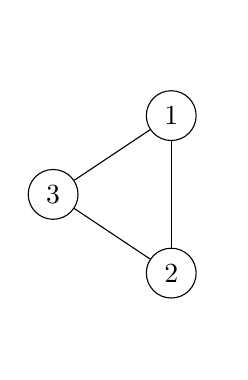
\begin{tikzpicture}
  \fill [white] (-1, -2) rectangle (1, 2) node {};  % Zentriere Graph.
  \tikzstyle{node}=[circle,draw, minimum width=18pt, inner sep=0pt, fill=white]

  \node[node] (1) at (-1,   0) {$3$};
  \node[node] (2) at (0.5,  1) {$1$};
  \node[node] (3) at (0.5, -1) {$2$};

  \path (1) edge (2);
  \path (1) edge (3);
  \path (2) edge (3);
\end{tikzpicture}
}
\hspace{1cm}
  \subfigure[Anorderung der Knoten zu einem binären Baum]{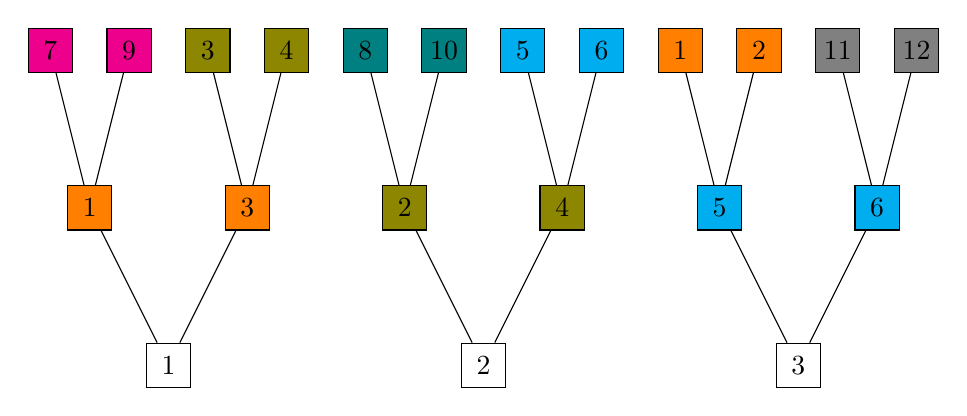
\begin{tikzpicture}
  \tikzstyle{node}=[rectangle,draw, minimum width=16pt, minimum height=16pt, inner sep=0pt, fill=white]
  \tikzstyle{color1}=[fill=orange]
  \tikzstyle{color2}=[fill=olive]
  \tikzstyle{color3}=[fill=cyan]
  \tikzstyle{color4}=[fill=magenta]
  \tikzstyle{color5}=[fill=teal]
  \tikzstyle{color6}=[fill=gray]

  \node[node, color4] (01)  at (-5.5, 2) {$7$};
  \node[node, color4] (02)  at (-4.5, 2) {$9$};
  \node[node, color2] (03)  at (-3.5, 2) {$3$};
  \node[node, color2] (04)  at (-2.5, 2) {$4$};
  \node[node, color5] (05)  at (-1.5, 2) {$8$};
  \node[node, color5] (06)  at (-0.5, 2) {$10$};
  \node[node, color3] (07)  at (0.5,  2) {$5$};
  \node[node, color3] (08)  at (1.5,  2) {$6$};
  \node[node, color1] (09)  at (2.5,  2) {$1$};
  \node[node, color1] (010) at (3.5,  2) {$2$};
  \node[node, color6] (011) at (4.5,  2) {$11$};
  \node[node, color6] (012) at (5.5,  2) {$12$};

  \node[node, color1] (11) at (-5, 0) {$1$};
  \node[node, color1] (12) at (-3, 0) {$3$};
  \node[node, color2] (13) at (-1, 0) {$2$};
  \node[node, color2] (14) at (1,  0) {$4$};
  \node[node, color3] (15) at (3,  0) {$5$};
  \node[node, color3] (16) at (5,  0) {$6$};

  \node[node] (21) at (-4, -2)  {$1$};
  \node[node] (22) at (0,  -2)  {$2$};
  \node[node] (23) at (4,  -2)  {$3$};

  \path (21) edge (11);
  \path (21) edge (12);
  \path (22) edge (13);
  \path (22) edge (14);
  \path (23) edge (15);
  \path (23) edge (16);
  \path (11) edge (01);
  \path (11) edge (02);
  \path (12) edge (03);
  \path (12) edge (04);
  \path (13) edge (05);
  \path (13) edge (06);
  \path (14) edge (07);
  \path (14) edge (08);
  \path (15) edge (09);
  \path (15) edge (010);
  \path (16) edge (011);
  \path (16) edge (012);
\end{tikzpicture}
}
\caption[Pooling auf Graphen]{Illustration einer Pooling-Operationen der Größe $4$ (\bzw{} zweier Pooling-Operationen der Größe $2$) auf einem Graphen \gls{G} der Größe $\left|\gls{V}\right| = 8$.
Das Clustering von \gls{G} liefert uns im ersten Schritt $N_1 =\left|\gls{V}_1\right| = 5$ Knoten und im darauf folgenden $N_2 = \left|\gls{V}_2\right| = 3$ Knoten.
Die Größen der Graphen werden daraufhin zu $N_2 = 3$, $N_1 = 6$ und $N_0 = 12$ angepasst, so dass jeder Knoten auf genau $2$ Vorgängerknoten verweist, indem \enquote{Fake}-Knoten zu $\gls{G}_1$ (1 Knoten) und $\gls{G}_0$ (4 Knoten) hinzugefügt werden.
Mit der Anordnung der Knoten zu einem binären Baum (d) kann die Pooling-Operation $\max\left(\cdot\right)$ eines Signals $\ve{f} \in \gls{R}^{12}$ auf $\gls{G}_0$ dann effizient als $\ve{f}_{\mathrm{pool}} \coloneqq {\left[ \max\left(\ve{f}_1, \ve{f}_2, \ve{f}_3, \ve{f}_4 \right), \max\left(\ve{f}_5, \ve{f}_6, \ve{f}_7, \ve{f}_8 \right), \max\left(\ve{f}_9, \ve{f}_{10}, \ve{f}_{11}, \ve{f}_{12} \right) \right]}^{\top} \in \gls{R}^3$ implementiert werden, wobei die Werte der \enquote{Fake}-Knoten $\ve{f}_2, \ve{f}_6, \ve{f}_{11}, \ve{f}_{12}$ auf den neutralen Wert $0$ der \gls{relu}-Aktivierungsfunktion gesetzt werden.}
\label{fig:pooling}
\end{figure}

\section{Netzarchitektur}
\label{raeumliche_netzarchitektur}

% Hier den Cube vorstellen
% 1D Convolutions etc

\begin{figure}[t]
\centering
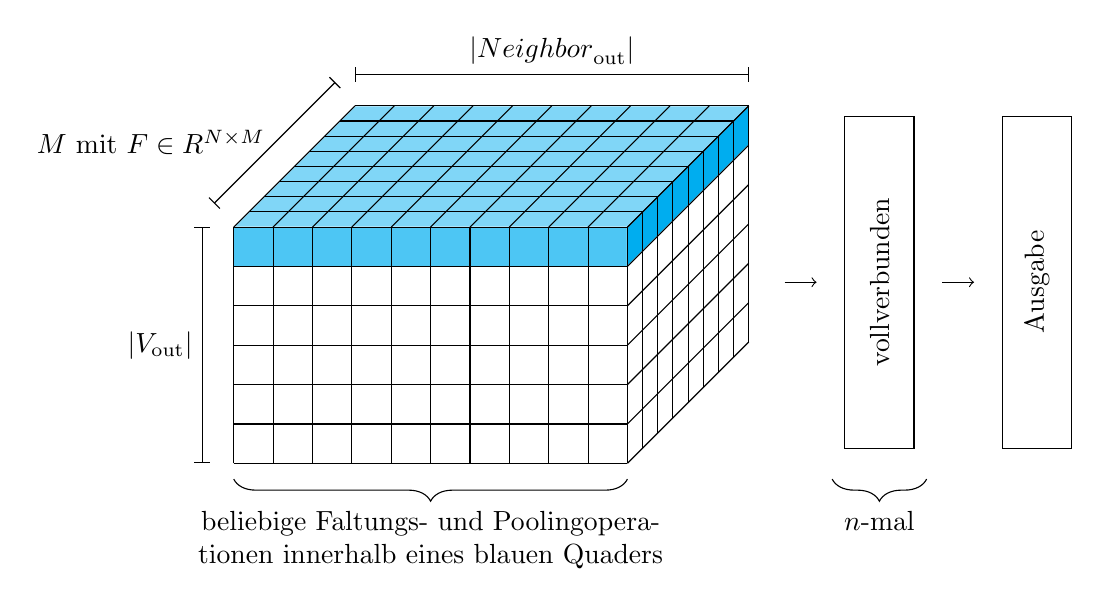
\begin{tikzpicture}
  \draw[white,fill=cyan!70] (0, 3, 4) -- (5, 3, 4) -- (5, 2.5, 4) -- (0, 2.5, 4) -- cycle;
  \draw[white,fill=cyan!50] (0, 3, 4) -- (5, 3, 4) -- (5, 3,   0) -- (0, 3,   0) -- cycle;
  \draw[white,fill=cyan]    (5, 3, 4) -- (5, 3, 0) -- (5, 2.5, 0) -- (5, 2.5, 4) -- cycle;
  \tikzstyle{path}=[->, shorten >= 10pt, shorten <= 10pt]
  \tikzstyle{node}=[rectangle,draw, minimum width=120pt, minimum height=25pt, inner sep=0pt, fill=white, rotate=90]
  \tikzstyle{noborder}=[draw=none,fill=none]

  \foreach \x in {0,0.5,1,1.5,2,2.5,3} {%
    \draw (0,  \x, 4)  -- (5,  \x, 4);
    \draw (5,  \x, 4)  -- (5,  \x, 0);
  }
  \foreach \x in {0,0.5,1,1.5,2,2.5,3,3.5,4,4.5,5} {%
    \draw (\x, 0,  4)  -- (\x, 3,  4);
    \draw (\x, 3,  4)  -- (\x, 3,  0);
  }
  \foreach \x in {0,0.5,1,1.5,2,2.5,3,3.5,4} {%
    \draw (5,  0,  \x) -- (5,  3, \x);
    \draw (0,  3,  \x) -- (5,  3, \x);
  }

  \draw[|-|] (-0.4, 0,    4)    -- node[left]  {$\left|\gls{V}_{\mathrm{out}}\right|$}        (-0.4, 3,    4);
  \draw[|-|] (0,    3.55, 4.65) -- node[left]  {$M$ mit $\ma{F} \in \gls{R}^{N \times M}$}    (0,    3.55, 0.65);
  \draw[|-|] (0,    3.4,  0)    -- node[above] {$\left|\gls{Neighbor}_{\mathrm{out}}\right|$} (5,    3.4,  0);

  \node[node, noborder] (0) at (6.2,  2.3, 4) {};
  \node[node]           (1) at (8.2,  2.3, 4) {vollverbunden};
  \node[node]           (2) at (10.2, 2.3, 4) {Ausgabe};

  \path[path] (0) edge (1);
  \path[path] (1) edge (2);

  \draw [decoration={brace,mirror,amplitude=8pt},decorate,-] (0,-0.2,4) -- node[below=8pt,text width=8cm, align=center] {beliebige Faltungs- und Poolingoperationen innerhalb eines blauen Quaders} (5,-0.2,4);
  \draw [decoration={brace,mirror,amplitude=8pt},decorate,-] (7.6,-0.2,4) -- node[below=8pt] {$n$-mal} (8.8,-0.2,4);

\end{tikzpicture}
\caption[Räumliche Netzarchitektur auf Graphen]{Typische räumliche Netzarchitektur auf Graphen.
Der \emph{Quader}, der durch die Anordnung der Knoten entsprechend ihrer Nachbarschaften entsteht, kann entlang der Nachbarschaften und ihrer Merkmale beliebig oft gefaltet und gepoolt werden.
Eine Faltung entlang der Knotenauswahl besitzt allerdings keine Bedeutung und ist deshalb zu vermeiden.
Im Anschluss können vollverbundene Schichten hin zur Ausgabe an den abgeflachten Quader gestapelt werden.}
\label{fig:netzarchitektur_raeumlich}
\end{figure}


Eigentliche Graphstruktur geht verloren (\zB{} Distanzen der Knoten zueinander) (in gewisser weise stecken diese aber in den Formfeatures).

Die Anordnung der Knoten zu einem Quaderform besitzt damit die Einschränkung, dass das Netz lediglich eine Faltungsschicht enthalten kann.
Die Methode der spektralen Faltung auf Graphen umgeht diese Einschränkung.

Würfel ist speicherineffizient

